\documentclass[10pt, a4paper]{article}
% especifico márgenes manualmente
\usepackage[paper=a4paper, left=1.5cm, right=1.5cm, bottom=1.5cm, top=3.5cm]{geometry}
% codificación ISO-8859-1
\usepackage[utf8]{inputenc}
%\usepackage[utf8x]{inputenc}
% separación silábica en castellano
\usepackage[spanish]{babel}
% utils
\usepackage{etoolbox,caption}
% paquetes y caratula de algo2
\usepackage{aed2-symb,aed2-itef,aed2-tad,aed2-newalgo,aed2-interfaz,caratula}
\usepackage{graphicx}
% hipervinculos en el indice
\usepackage{hyperref}
% algoritmos
\usepackage{algorithm}
\usepackage{algorithmicx}
\usepackage{algpseudocode}
\usepackage{amsmath}
\usepackage{amsfonts}


\parskip=5pt % 10pt es el tamaño de fuente

\begin{document}

% Estos comandos deben ir antes del \maketitle
\materia{Algoritmos y Estructuras de Datos III} % obligatorio
\submateria{Primer Cuatrimestre de 2017} % opcional
\titulo{Trabajo Práctico 2} % obligatorio
%\grupo{Grupo} % opcional

\integrante{Salvador, Alejo}{467/15}{alelucmdp@hotmail.com} % obligatorio 


\maketitle

% compilar 2 veces para actualizar las referencias
\tableofcontents

\pagebreak
\section{Ejercicio 2}

\subsection{Descripción del problema}

\subsubsection{Enunciado Informal}

En este problema se nos presenta un conjunto de ciudades con rutas entre las mismas que van en una sola dirección. No necesariamente se puede llegar desde una ciudad a cualquier otra pero necesariamente toda ciudad debe tener al menos una ciudad a la que se pueda viajar.
Cada una de las rutas tiene un determinado costo para realizar el viaje. Se desea reducir el costo de viajar en todas las rutas por un costo fijo C (puede llevar a que el costo de viajar en una ruta sea negativo). Se desea hallar el maximo C tal que no hay una camino que empieze en una ciudad y vuelva a esa misma ciudad con un costo total negativo.  

\subsubsection{Enunciado Formal}

Se tiene un grafo dirigido que no tiene ningun vertice de grado 0. Cada una de las aristas tiene pero determinado. Se desde hallar el maximo C tal que se reduce el peso de todas las aristas por ese valor fijo C (puede pasar a haber aristas con peso negativo), tal que no pase a haber ningun ciclo con peso total negativo.

\subsubsection{Formato de entrada y salida}
La entrada esta conformada por:\\
una línea con 2 entero N  y M con la cantidad de ciudades y de de rutas respectivamente;\\
M lineas con enteros c1 y c2 que indican cuales ciudades comunica la ruta a describir en la linea, seguido de un entero positivo P indicando el costo de viajar por la misma.
\\
La salida es un único entero Solución con el máximo valor por el cual se pueden disminuir todos los peajes.

\subsubsection{Ejemplos con Soluciones}
Ejemplo:un ejemplo en que no queda ningun elemento sin pintar\\
Entrada:\\
4 5\\
0 1 3\\
1 2 1\\
2 1 2\\
0 3 6\\
3 0 4\\
Salida:\\
2\\
Explicacion:\\
En este grafo se presentan 2 ciclos que son el que va a 3 en un proceso de ida y vuelta al cual se le podria restar hasta 5, y el otro ciclo es que va de 0-1-2-3-0, al cual se le puede restar 2 porque el costo total del viaje termina en 0 pero si le restar 3 terminaria en -3. Entonces únicamente se puede restar hasta 2. Cualquier otro ciclo que incluya que vuelva hasta el punto de origen y luego vuelva a viajar por otro recorrido no sirve porque literalmente serian 2 ciclos en 1 y su costo sería la suma de los 2 costos por lo que NO sería negativo al menos que uno de los 2 sea ya negativo.



\subsection{Explicación de la solución}

 Primero es importante notar que no puede pasar que no existan ciclos en el grafo ya que al tener al menos una arista saliendo de cada vertice si se va siguiendo un camino partiendo de una arista cualquiera, el camino nunca puede terminar en un punto muerto, por lo que necesariamente deberá formarse un ciclo. En conclusión todo arista debe pertenecer a al menos un ciclo. Por lo tanto si tuviera todas las aristas negativas tendríaa todos los caminos negativos y al menos uno de ellos sería un ciclo. Entonces ya se sabe que no se puede restar más que el peso de la arista de mayor peso. Hallar la arista de mayor peso es muy rapido ya que solo se debe recorrer todas una vez teniendo una complejidad final de \bigo(M)\\
Ahora ya establecido lo anterior, para resolver este problema es importante mecionar que el algoritmo de Belman-Ford \url{https://en.wikipedia.org/wiki/Bellman–Ford_algorithm} es capaz de identificar todos los ciclos negativos que involucren vertices que son alcanzables desde el vertice desde el que parte el algoritmo y el mismo tiene complejiiad en el peor caso de \bigo(A*M), donde A es la cantidad de vertices alcanzables desde el vertice del que se partió. Esto es util ya que si se logra partir el bellman ford desde un conjunto de vertices tales que se logre cubrir la totalidad de los vertices del grafo exactamente una vez entonces se tendría un algoritmo con complejidad total \bigo(N*M) capaz de identificar en cualquier grafo dirigido, la presencia de un ciclo negativo. Para hacer esto se hará que cada iteración de bellman ford guarda la lista de vértices que fueron alcanzados desde el vértice original (es decir los vértices tales que al final del bellman ford la distancia que tiene al vertice original sea menos que infinito) y si el vértice fue previamente vistitado en otra itreación de bellman ford se ingorarán todas las aristas que lo involucren. Esto permite que no se vuelvan a recorrer los ciclos partiendo desde un vértice que ya fue incluido (ya que hallar los caminos de A a B y de B a C va a incluir los caminos de B a C). Al hacer esto cada vértice a lo sumo será visitado una vez. Ademas para evitar correr N-1 pasos en cada Bellman ford se realizara una pequeñá modificacion por la cual se dejara de intentar actualizar las distancias cuando la cantidad de pasos que se realizo en el bellman ford supere la cantidad de vertices alcanzados (ya que no puede haber ningún camino mas largo que la cantidad de vertices del mismisimo conjunto de vertices alcanzables). Por lo tanto al final de esto se correr varios bellman ford intentando partir de todos los vertices sucesivamente (si ya fue incluido como parte de los visitable desde una anterior ese vertice será ignorado) de modo tal que se encontrarán todos los ciclos negativos sin necesidad de incluir ningún vertice en 2 bellman ford distinto. Por lo tanto este paso termino teniendo una complejidad de \bigo(N*M) como era buscado.\\
Ahora teniendo esto solo resta hacer una busqueda binaria donde se pruebe restar los distintos valores para restar (son menores o iguales a K por lo explicado al principio) y hallar el máximo valor de k tal que la combinación de Bellman-Ford no incluya ningun ciclo negativo. Por lo tanto al estar usando busqueda binaria solo se deben probar log(K) valores posibles para restar. Como tenemos que para cada valor a probar se necesita correr un algoritmo de complejidad \bigo(N*M) se tiene que la complejidad final sería \bigo(N*M*log(K)) lo cual es exactamente la complejidad pedida.\\


Para el pseudocodigo se utilizara una función que se encarga por su cuenta de hacer Bellman-Ford mientras que el codigo princial search solution se encargaria de hacer la busqueda binaria e ir haciendo los llamados a bellman ford . Ademas el vector edges tine tuplas que indicar los 2 vertices de la lista c1 c2 siendo c1 el de origen y c2 el de llegada. Mientras tanto el tercer elmento de la tupla es el peso de dicha arista.



	\algoritmo{searchsolution}{entero n,entero m, $vector<tupla<entero, entero,entero>> edges$}{entero}{\bigo($N*M*log(K)$)}{
	
\State Max $\gets$ 0 \comment \bigo($1$)	
\For {i $\gets edges[0],edges[1],...,edges[m-1]$} \comment se repite m veces
\State Max $\gets$ maximo(max,i[2]) \comment \bigo($1$)

\EndFor	

\If {$max=0$}  \comment \bigo($1$)
	\State devolver 0 \comment \bigo($1$)
\EndIf


\If {$max>0$}  \comment \bigo($1$)

\State $limiteizquierdo \gets -1$ \comment \bigo($1$)
\State $limitederecho \gets max+1$ \comment \bigo($1$)
\While {$limitederecho - limiteizquierdo > 1$} \comment se repite a lo sumo log(k) veces por ser una busqueda binaria)
	\State $medio \gets limiteizquierdo+ (limitederecho-limiteizquierdo)/2$ \comment \bigo($1$)
	\If {$bellmanford(n,m,edges,-medio)=true$} \bigo($n*m$)
		\State $limitederecho \gets medio$ \comment \bigo($1$)
	\EndIf
		\If {$bellmanford(n,m,edges,-medio)=false$} \bigo($n*m$)
		\State $limiteizquierdo \gets medio$ \comment \bigo($1$)
	\EndIf


\EndWhile
\State devolver limite izquierdo
\EndIf
	

 
}{\bigo(M)$+log(k)*2 $\bigo(N*M)}


\algoritmo{bellmanford}{entero n,entero m, $vector<tupla<entero, entero,entero>> edges$,entero modificador}{entero}{\bigo($N*M$)}{
	
	\State respuesta $gets$ FALSE
\State Crear visitado que es arreglo que indica si fue visitado el vertice. Empizan todos en no visitados 	
\For {i $\gets $ 0,1,...n-1} 

\If {$visitado[i]=FALSE$}  
\State visitado[i] $\gets$ TRUE
	\State Crear distancia que es arreglo que indica la distancia de cada vertice al vertice de origen i. Empizan todos en infinito 
	\State distancia[0] $\gets$ 0
	\State Ivertex $\gets$ 0
	\State limit $\gets$ 1
	\State distanceModifired $\gets$ TRUE
	\While {$distanceModified=TRUE \wedge Ivertex<limit$}
		\State distanceModified $\gets$ FALSE
		\For {edge $\gets$ edges[0],edges[1],...,edges[m-1] }
			\State edgeweight $\gets edge[2]+modificador$
			\State v1 $\gets edge[0]$
			\State v2 $\gets edge[1]$
		
			\If {$distancia[v1]\neq INFINITO \wedge distancia[v1]+edgeweight<distance[v2] \wedge visitado[i]=FALSE$}
			\State $limit \gets limit+1$
			\State $visitado[v2] \gets TRUE$
			\State $distancia[v2] \gets distancia[v1]+edgeweight$
			\State distanceModified $\gets TRUE$
			\EndIf
		\EndFor
	
		\State Ivertex $\gets$Ivertex+1
	\EndWhile	
	
	\If {Ivertex=limit}	
		\State respuesta $\gets$TRUE
	
	\EndIf
		
\EndIf


\EndFor	
\State devolver respuesta



	

 
}{}





\pagebreak
\newpage
\section{Ejercicio 3}

\subsection{Descripción del problema}

\subsubsection{Enunciado Informal}

En este problema se nos presenta un conjunto de ciudades con rutas entre las mismas que pueden o no estar ya construidas y tienen un costo de construccion/destrucción dependiendo de si ya existen. Se debe destruir y construir rutas tal que haya una sola forma de llegar de una ciudad a cualquier otra (se puede pasar por ciudades intermedias).Se debe tratar de minimzar el costo de conseguir este objetivo.

\subsubsection{Enunciado Formal}

Se tiene un conjunto de vertices y aristas que conectan a algunos de estos vertices entre si. Para cada par de vertices existen un número asignado el cual es el costo de agregar/eliminar la arista que conecta estos 2 vecrtices. El objetivo es encontrar el minimo coste necesario para lograr que el grafo resultante sea un arbol de expansión.\\
Esto es equivalente al enunciado orginal porque los vertices son las ciudades, los caminos son las aristas y la definición de arbol de expansión es un árbol que incluya todos los vertices del grafo (y la definición de árbol es que haya exctamente una única manera de llegar de un vertice a cualquier otro del mismo).

\subsubsection{Formato de entrada y salida}
La entrada esta conformada por:\\
una línea con un entero N con la cantidad de ciudades;\\
N*(N-1)/2 lineas describiendo como estan comunicados 2 ciudades.
Estas lineas estan formados por 2 enteros C1 y C2 indicando la conexión entre que par de vertices se está describiendo, seguido de un entero E indicando si la ruta existe y un entero P indicando el costo de construcción/destrucción de la ruta.\\
La salida es una unica linea con un entero indicando el minimo costo requerido para lograr el objetivo, seguido de un entero con la cantidad de rutas que forman parte de la solución y la lista de rutas que forman parte de la solución descriptas como un par de enteros que indican el par de ciudades que esa ruta conecta

\subsubsection{Ejemplos con Soluciones}
Ejemplo:un ejemplo en que no queda ningun elemento sin pintar\\
Entrada:\\
4\\
0 1 0 3\\
0 2 0 1\\
1 2 1 2\\
0 3 0 6\\
1 3 1 4\\
2 3 1 1\\
Salida:\\
2 3 0 3 1 3 0 2\\
Explicacion:\\
Como 1 2 y 3 forman un triangulo con todo conectado necesariamente se debe eliminar una arista. Se elimará la mas barata ya que el objetivo es simplemente incluir todos los elementos con el menor costo posible. Asi que no conviene gastar en eliminar demás ni en agregar en exceso. Si que es necesario elminar exactamente 1 y esa sería la arista mas barata (es decir la de costo 1. De manera similar el vertice 0 quedo aislado del grafo y debe comunicarse usando el camino mas corto posible el cual tiene costo 1.




\subsection{Explicación de la solución}

Para resolver este problema es importante notar que si divido el grafo original en sus componentes conexas, se puede notar que las únicas operaciones permitidas serían eliminar aristas dentro de cada componente o agregar para conectar las componentes. Es obvio que las compnentes al ser conexas no tienen caminos conectandolas por lo cual es obvio que solo se puede agregar aristas por lo tanto lo único que sería demostrar es la otra afimación\\
 Esto es así ya que agregar aristas dentro de un mismo componente lo único que hace es agregar mas aristas a las posibles para eliminar, ya que se crean caminos alternativos y agrega aristas al total. Esto en principio podría ser positivo ya que podría haber una combinación de agregar una arista y eliminar 2 que sea más óptima que eliminar una sola. Sin embargo, esto no es asi ya que al agregar aristas únicamente se permite eliminar aristas que comunican 2 vertices que previamente estaban comunicados con un conjunto de caminos que tienen exactamente una arista que se encuentra en todos los caminos (pero con la arista extra tienen caminos alternativos que no usan dicha arista), ya que caulquier otra arista ya anteriormente podía ser eliminada. Es decir 2 conjuntos de vertices cada uno de los cuales tienen al menos 2 caminos entre cada par de vértices del mismo pero solo uno a los del otro conjunto. Si se agrega una arista dentro de un conjunto este no se ve afectado (de la misma manera si agrega una con alguno fuera de estos conjuntos no se crea ningún camino alternativo), pero si se agreaga una arista comunicando los 2 conjuntos distintos se crea la posibilidad de elegir alguno de los 2 caminos comunicando los conjuntos. Como cada arista agregada solo puedo afectar a un par de estos conjuntos (ya que ninguna pueda estar afuera) a lo sumo es posible crear un camino nuevo. En caso de que el camino orignal este formado por varios elementos se sabe que debe esta formado por todas aristas que no tienen otra forma de comunicarse a la totalidad de los vertices sin usar dicho camino ya que si lo hubiera existiría otro camino alternativo entre los 2 conjuntos originales. Por lo tanto solo es posible eminar una arista de dicho camino. Por lo tanto al agregar una arista se debe eliminar una arista extra para mantener el total pero se permite eliminar a lo sumo 1 arista que previamente no podía serlo. En conclusión se debe seguir elimando la misma cantidad de aristas de las originales y solo se aumenta el costo total agregando y elminando una demás \\
Entonces ya sabiendo que solo se puede realizar esas operaciones el problema se redujo en varios subproblemas en lo que se debe formar su arbol de máxima expansión ya que de esa manera se minimiza el costo de las aristas no usadas. Esto se puede hacer en pasos consistenes en agreagar a dicho arbol la arista de maximo tamaño posible en cada paso que no conecte vertices previamente conectados. Esto es exactamente lo que hace el algoritmo de kruskal \url{https://es.wikipedia.org/wiki/Algoritmo_de_Kruskal} el cuál será implementado teniendo un arreglo ordenado de forma decreciente con todas las aristas destruibles de la componente conexa con la que se esta trabajando. Al agregar una arista a dicho arbol es importante guardar cual fue la arista agregada para así poder reconstruir la solución para la salida. Cuando no se agrega una arista porque comunica 2 vertices ya previamente conectadas se le suma el valor correspondiente al costo total de las obras. Notese que se puede trabajar directamente con otdas las componentes fuertemente conexas a la vez en el mismo arreglo ya que simplemente haría que se vaya trabajando con cada subproblema por partes ya que no estan comunicados de ninguna manera\\
Ahora solo quedaría conectar todas dichas componentes. Para hacer eso se debe hacer un arbol que conecte la otdalidad de los nodos tratando de minimizar el costo. Para hacer esto también se podra usar kruskal pero suponiendo que cada una de las componentes conexas ya estan conectadas y cada una forman su propio conjunto en el algooritmo (sería parecido a empezar el algoritmo por la mitad del mismo). Para hacer esto se tomará las aristas construibles y se colocaran en un arreglo ordenado de forma creciente de tal manera que en cada paso se tome la de menor costo y se agregará al arbol generador final en caso que conecte 2 verticces que previamente no estaban comunicados entre si. De la misma forma que en el caso anterior cada vez que se agrega una arista se aumentariá el costo total y guardará la arista agregada para reconstruir la solución\\


Para el psudocodigo se utilizará la función sort que ordena el vector dado de menor a mayor o mayor a menor. La misma tiene complejidad en el peor caso de N*log(N) ya que la misma en las biblotecas standard por mas que varíen implementación deben garantizar un peor caso de N*log(N). Luego de leer la entrada lo cual se hace en tiempo O(1) para cada una de las n*(n-1)/2 lineas (ya que solo se debe colocar la información en el vector conrrespondiente), se procederá a resolver el problema con la información correspondiente ya colocada en los vectores destruction y construction (de acuerdo si el camino ya existe o no) guardando en cada una la tupla formada por c1, c2 y costo P. Por lo tanto construction como destruction pueden tener a lo sumo un elemento por linea de codigo por lo cual pueden tener a lo sumo O(N*N) elementos. Además es importante mencionar que de utilizará una clase llamada disjoint set que es un conjunto de elementos divido en varios subconjuntos implementada utilizando union find \url{https://en.wikipedia.org/wiki/Disjoint-set_data_structure} la implentación usada tiene complejidad de O(N) tanto para construirse, destruirse, hacer el find y el union.Por lo tanto el pseudocodigo quedaría:



	\algoritmo{MenorCosto}{entero n, $vector<tupla<entero, entero, entero>> construction$, $vector<tupla<entero, entero, entero>> destruction$}{}{\bigo($N*N*log(N)$)}{
	
\State sortcreciente(construction)\comment \bigo($N*N*log(N)$)
	\State sortdecreciente(destruction)\comment \bigo($N*N*log(N)$)
	\State Crear DisjointSet UDS de tamaño N \comment \bigo($N$)
	
\State Minimo $\gets$ 0 \comment \bigo($1$)
\State $vector<tupla<entero, entero>> solucion$
\For {i $\gets destruction[0],destruction[1],...,destruction[tamano(destruccion)-1]$} \comment se repite a lo sumo N*N veces
\State v1 $\gets$ i[0] \comment \bigo($1$)
\State v2 $\gets$ i[1] \comment \bigo($1$)

\If {$UDS.find(v1)\neq UDS.find(v2)$} \comment \bigo($N$)
	\State $UDS.setUnion(v1, v2)$; \comment \bigo($N$)
	\State Agregar $(v1,v2)$ al vector solucion  \comment \bigo($1$)
\EndIf
\If {$UDS.find(v1) = UDS.find(v2)$} \comment \bigo($N$)
	\State Minimo $\gets$ $Minimo-i[3]$; \comment \bigo($1$)
\EndIf

\EndFor

\For {i $\gets construction[0],construction[1],...,construction[tamano(construccion)-1]$} \comment se repite a lo sumo N*N veces
\State v1 $\gets$ i[0] \comment \bigo($1$)
\State v2 $\gets$ i[1] \comment \bigo($1$)

\If {$UDS.find(v1)\neq UDS.find(v2)$} \comment \bigo($N$)
	\State $UDS.setUnion(v1, v2)$; \comment \bigo($N$)
	\State Agregar $(v1,v2)$ al vector solución \comment \bigo($1$)
	\State Minimo $\gets$ $Minimo-i[3]$;\comment \bigo($1$)
\EndIf
\EndFor
	
\State la solución es Minimo seguido de n-1 y por ultima el contenido del vector solución escribiendo los elementos de cada par uno despues del otro.   
   
 
}{\bigo(N*N*log(N)) + \bigo(N*N)+\bigo(N*N)$=$\bigo(N*N*log(N))}


\subsection{Experimentación}
La experimentación del ejercicio 3 se llevó a cabo armando un grafo completo completo de n nodos. Las aristas se generaron desde (v1, v2), (v2, v3), ..., (v2, v3), (v3, v4), ..., (v(n-1), v(n-2)). Los costos son completamente aleatorios en cada instancia generada, para demostrar que no afectan los tiempos de ejecución, y para asignarle una densidad al grafo, se ordenó la lista de incidencia de manera aleatoria y se tomaron los max m * densidad primeros elementos de la mismas.\\
 
La principal observación que se puede realizar para este algoritmo es que los tiempos de ejecución dependen enteramente de la cantidad de vértices. La dependencia en N es visible en el cálculo de complejidad, pero se puede corroborar que cualquier variación de instancias no modifica los tiempos de ejecución. Para esto variamos la densidad del grafo, tomando aristas y costos de construcción completamente aleatorios para cada una, pero con N fijo. Esto nos da una distribución normal lo que nos permite corroborar que ninguna otra característica del grafo afecta los tiempos de ejecución:\\


\begin{figure}[!htb!]
	\begin{center}
		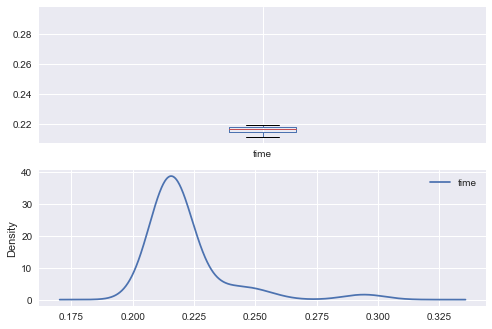
\includegraphics[width=300pt]{Imagenes/density.png}
		\caption{{\small \textit{densidad}}}
	\end{center}
\end{figure}




\end{document}